\documentclass[11pt]{article}

\usepackage{tikz}

\usepackage{my_notes}

\begin{document}
	\title{Electricity \& Magnetism Notes}
	\author{Sean Richardson}
	\date{\today}
	\maketitle
	
	\raggedright
	
	\section{???}
		There exists \textbf{charge}
		\begin{myitems}
			\item 2 varieties $(+,-)$
			\item Conserved
			\item Can be transferred by rubbing (triboelectric effect)
			\item Can produce both attractive and repulsive forces
			\item Quantized (discrete amounts)
			\begin{myitems}
				\item Smallest charge: $e=1.6\times 10^{-19} C$. A proton has charge $+e$, and an electron has charge $-e$. (No idea why these are the same)
			\end{myitems}
		\end{myitems}
		\subsection{Coulomb's Law}
			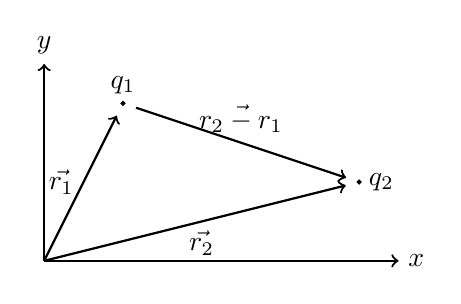
\begin{tikzpicture}
				%defs
				\def\dist{5pt}
				\def\rad{0.025}
				\coordinate (o) at (0,0);
				\coordinate (Y) at (0,2.5);
				\coordinate (X) at (4.5,0);
				\coordinate (1) at (1,2);
				\coordinate (2) at (4,1);
				%dots
				\draw[fill] (1) circle [radius=\rad];
				\draw[fill] (2) circle [radius=\rad];
				%lines
				\draw [thick, ->] (o) -- (Y);
				\draw [thick, ->] (o) -- (X);
				\draw [thick, ->, shorten >= \dist] (o) -- (1);
				\draw [thick, ->, shorten >= \dist] (o) -- (2);
				\draw [thick, ->, shorten >= \dist, shorten <= \dist] (1) -- (2);
				%Labels
				\node[above] at (1) {$q_1$};
				\node[right] at (2) {$q_2$};
				\node[above] at (Y) {$y$};
				\node[right] at (X) {$x$};
				\node[left] at (0.5,1) {$\vec{r_1}$};
				\node[below] at (2,0.5) {$\vec{r_2}$};
				\node[above] at (2.5,1.5) {$\vec{r_2-r_1}$};
			\end{tikzpicture}
			\begin{equation}
				\vec{F}_{12} = \frac{k q_1 q_2}{r_{12}^2}\hat{r}_{12}
			\end{equation}
			\section{Constants}
				\begin{mydes}
					\item{$m_e$:} $9.11 \times 10^{-31} kg$
					\item{$q_e$:} $1.60 \times 10^{-19} C$
				\end{mydes}
\end{document}